\documentclass[export, 12pt, letterpaper]{ctexrep}

\usepackage{titling}
\usepackage{standalone}
\usepackage{fontenc}


\usepackage[x11names]{xcolor}
\definecolor{SaddleBrown}{rgb}{0.55, 0.27, 0.07}
\definecolor{IndianRed}{rgb}{0.80, 0.36, 0.36}
\definecolor{Firebrick}{rgb}{0.70, 0.13, 0.13}
\definecolor{DarkBlue}{rgb}{0, 0, 0.55}
\definecolor{Goldenrod}{rgb}{0.85, 0.65, 0.13}
\definecolor{Peru}{rgb}{0.85, 0.65, 0.13}




\usepackage{hyperref}
\hypersetup{
    colorlinks=true,
    linkcolor=DarkBlue,
    urlcolor=blue,
    filecolor=DarkBlue,
    linktoc=all
}
\setcounter{tocdepth}{1}


\usepackage{mathtools}
\usepackage{amsmath}
\usepackage{tikz}
\usepackage{verbatim}
\usetikzlibrary{calc}
\usetikzlibrary{shapes.geometric}

% put color to \boxed math command
\newcommand*{\boxcolor}{Peru}
\makeatletter
\renewcommand{\boxed}[1]{\textcolor{\boxcolor}{%
\tikz[baseline={([yshift=-1ex]current bounding box.center)}] \node [rectangle, minimum width=1ex,rounded corners,draw] {\normalcolor\m@th$\displaystyle#1$};}}
\makeatother


\usepackage{listings}

\definecolor{codegreen}{rgb}{0,0.6,0}
\definecolor{codegray}{rgb}{0.5,0.5,0.5}
\definecolor{codepurple}{rgb}{0.58,0,0.82}
\definecolor{backcolour}{rgb}{0.95,0.95,0.92}

\lstdefinestyle{mystyle}{
    backgroundcolor=\color{backcolour},
    commentstyle=\color{codegreen},
    keywordstyle=\color{magenta},
    numberstyle=\tiny\color{codegray},
    stringstyle=\color{codepurple},
    basicstyle=\ttfamily\footnotesize,
    breakatwhitespace=false,
    breaklines=true,
    captionpos=b,
    keepspaces=true,
    numbers=left,
    numbersep=5pt,
    showspaces=false,
    showstringspaces=false,
    showtabs=false,
    tabsize=2
}

\lstset{style=mystyle}


\usetikzlibrary{positioning}
\usetikzlibrary{petri} % LATEX and plain TEX
\usetikzlibrary[petri] % ConTEXt
\usepackage{pgfplots}
\pgfplotsset{compat=1.13}


\usepackage{framed}
\usepackage{quoting}

\colorlet{shadecolor}{LightSteelBlue1}
\usepackage{lipsum}
\newenvironment{shadedquotation}
 {\begin{shaded*}
  \quoting[leftmargin=5pt, rightmargin=5pt, vskip=0pt]
 }
 {\endquoting
 \end{shaded*}
}


\usepackage{lipsum} % for dummy text
\usepackage{enumitem}
\setlist{nosep} % or \setlist{noitemsep} to leave space around whole list


\usepackage{graphicx}
\usepackage{adjustbox}
\usepackage{caption}
\usepackage{float}

\pagestyle{plain}

        

\usepackage{ctex}
\usepackage{xeCJK}
\xeCJKsetup{CJKmath=true}


            \usepackage[
                left=1.0in,
                right=1.0in,
                top=1.5in,
                bottom=1.5in,
            ]{geometry}
        

\setlength{\droptitle}{-18em}
\title{\fontsize{40}{20} \textbf{\textcolor{red}{\kaishu 桌游类小游戏开发框架}}}
\author{\textcolor{red}{南方小智}}
\date{\textcolor{red}{\today}}



\begin{document}

\maketitle
\thispagestyle{empty}
\newpage

\setcounter{page}{1}
\tableofcontents
\newpage

\begin{center}

\begin{picture}(500,544)

\put(0,0){\hbox{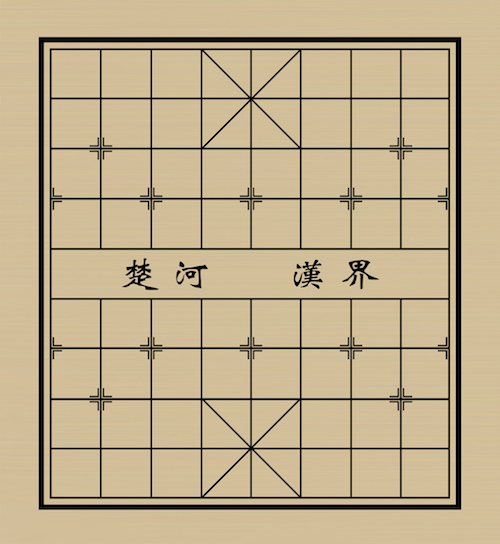
\includegraphics[scale=1]{wiki/images/ch_chess/board/board.png}}}

\put( 25, 20){\hbox{
\includegraphics[]{wiki/images/ch_chess/chess/r_ju.png}}}
\put( 75, 20){\hbox{
\includegraphics[]{wiki/images/ch_chess/chess/r_ma.png}}}
\put(125, 20){\hbox{
\includegraphics[]{wiki/images/ch_chess/chess/r_xiang.png}}}
\put(175, 20){\hbox{
\includegraphics[]{wiki/images/ch_chess/chess/r_shi.png}}}
\put(225, 20){\hbox{
\includegraphics[]{wiki/images/ch_chess/chess/r_jiang.png}}}
\put(275, 20){\hbox{
\includegraphics[]{wiki/images/ch_chess/chess/r_shi.png}}}
\put(325, 20){\hbox{
\includegraphics[]{wiki/images/ch_chess/chess/r_xiang.png}}}
\put(375, 20){\hbox{
\includegraphics[]{wiki/images/ch_chess/chess/r_ma.png}}}
\put(425, 20){\hbox{
\includegraphics[]{wiki/images/ch_chess/chess/r_ju.png}}}

\put( 75, 120){\hbox{
\includegraphics[]{wiki/images/ch_chess/chess/r_pao.png}}}
\put(375, 120){\hbox{
\includegraphics[]{wiki/images/ch_chess/chess/r_pao.png}}}

\put( 25, 170){\hbox{
\includegraphics[]{wiki/images/ch_chess/chess/r_zu.png}}}
\put(125, 170){\hbox{
\includegraphics[]{wiki/images/ch_chess/chess/r_zu.png}}}
\put(225, 170){\hbox{
\includegraphics[]{wiki/images/ch_chess/chess/r_zu.png}}}
\put(325, 170){\hbox{
\includegraphics[]{wiki/images/ch_chess/chess/r_zu.png}}}
\put(425, 170){\hbox{
\includegraphics[]{wiki/images/ch_chess/chess/r_zu.png}}}


\put( 25, 470){\hbox{
\includegraphics[]{wiki/images/ch_chess/chess/b_ju.png}}}
\put( 75, 470){\hbox{
\includegraphics[]{wiki/images/ch_chess/chess/b_ma.png}}}
\put(125, 470){\hbox{
\includegraphics[]{wiki/images/ch_chess/chess/b_xiang.png}}}
\put(175, 470){\hbox{
\includegraphics[]{wiki/images/ch_chess/chess/b_shi.png}}}
\put(225, 470){\hbox{
\includegraphics[]{wiki/images/ch_chess/chess/b_jiang.png}}}
\put(275, 470){\hbox{
\includegraphics[]{wiki/images/ch_chess/chess/b_shi.png}}}
\put(325, 470){\hbox{
\includegraphics[]{wiki/images/ch_chess/chess/b_xiang.png}}}
\put(375, 470){\hbox{
\includegraphics[]{wiki/images/ch_chess/chess/b_ma.png}}}
\put(425, 470){\hbox{
\includegraphics[]{wiki/images/ch_chess/chess/b_ju.png}}}

\put( 75, 370){\hbox{
\includegraphics[]{wiki/images/ch_chess/chess/b_pao.png}}}
\put(375, 370){\hbox{
\includegraphics[]{wiki/images/ch_chess/chess/b_pao.png}}}

\put( 25, 320){\hbox{
\includegraphics[]{wiki/images/ch_chess/chess/b_zu.png}}}
\put(125, 320){\hbox{
\includegraphics[]{wiki/images/ch_chess/chess/b_zu.png}}}
\put(225, 320){\hbox{
\includegraphics[]{wiki/images/ch_chess/chess/b_zu.png}}}
\put(325, 320){\hbox{
\includegraphics[]{wiki/images/ch_chess/chess/b_zu.png}}}
\put(425, 320){\hbox{
\includegraphics[]{wiki/images/ch_chess/chess/b_zu.png}}}


\end{picture}

\end{center}


\chapter{概述}

本项目用于实现各类桌游小游戏的游戏流程,AI玩家,对弈平台等。目前正在开发中国象棋的基本游戏流程和AI算法。

\section{安装与设置}
\begin{lstlisting}[language=Bash]
python3 -m pip install termcolor
\end{lstlisting}

\chapter{基本元素}

\begin{center}\begin{figure}[H] \centering 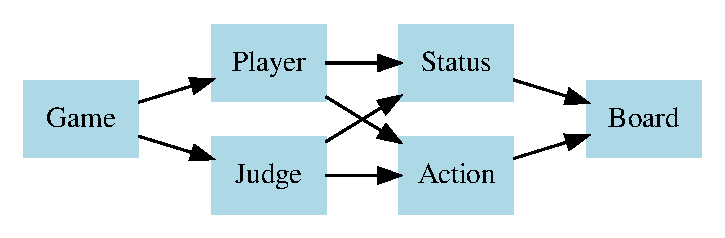
\includegraphics[max size={\textwidth}{\textheight},keepaspectratio]
{wiki/images/image1.dot.eps}\caption*{桌游小游戏基本元素}
\end{figure} \end{center}

游戏中的基本元素有,Board,Status,Action,Player,Judge,Game等。外部程序通过设置Game,Players,和Config,可以调用该框架。

\section{Board}

游戏中最基本的元素是Board,相当与棋盘,牌桌。其中包含各类游戏物件以及他们的位置,比如棋子,纸牌和骰子等。

Board提供对这些游戏物件的访问和改变,比如改变某个物件的位置。同时也对Board上的基本状态进行检测,比如在中国象棋中判断当前局面上将帅是否照面。

\section{Action}

Action代表某个玩家可以在Board上的一个操作。比如把某个子移动到另一个地方,称为MoveAction。可以通过继承Action实现更高级的动作,比如悔棋操作。MoveAction应当是可以撤销的(roll\_back),这样可以支持悔棋的功能,以及在AI搜索算法中可以利用其实现回溯。

认输也可以是一个Action。

\section{Status}

当前游戏的所有状态,包括Board的格局,当前玩家,获胜玩家,Action的历史栈等。
获得Status就可以知道游戏从初始到现在所有的需要的状态数据,也就是可以通过Status对整个游戏过程进行复盘。

\section{Player}

Player的主要任务是,在自己为主的一轮当中,通过当前的Status,按照顺序作出一个或多个Action。

Player可以是自动的AIPlayer,也可以接收输入的真人玩家,网络玩家等。

\section{Judge}

Judge负责判定Player产生的Action是否合法,并最终负责执行合法的Action。Judge还负责判断游戏是否已经结束,谁是胜利玩家等。Judge通过Rule来进行这些判定,不同的Rule集合可以产生略微不同的游戏规则,比如,可以在象棋中去掉将帅不可照面的规则等。

某些特殊的中国象棋残局添加了额外的限定,这种Judge和Rule解耦分开处理的方式有利于实现这些残局游戏。

Judge还可以用于控制游戏状态和流程,比如实现回退,保存局面等。

\section{Game}

Game控制整个游戏的流程,每个游戏由准备阶段开始,然后经过若干轮,每轮以其中一位Player为主,并由Judge执行操作。最后利用Judge判断游戏结束和得出胜利玩家列表。

\chapter{卡坦岛设计}

\section{游戏状态转换}

 \begin{center}\begin{figure}[H] \centering 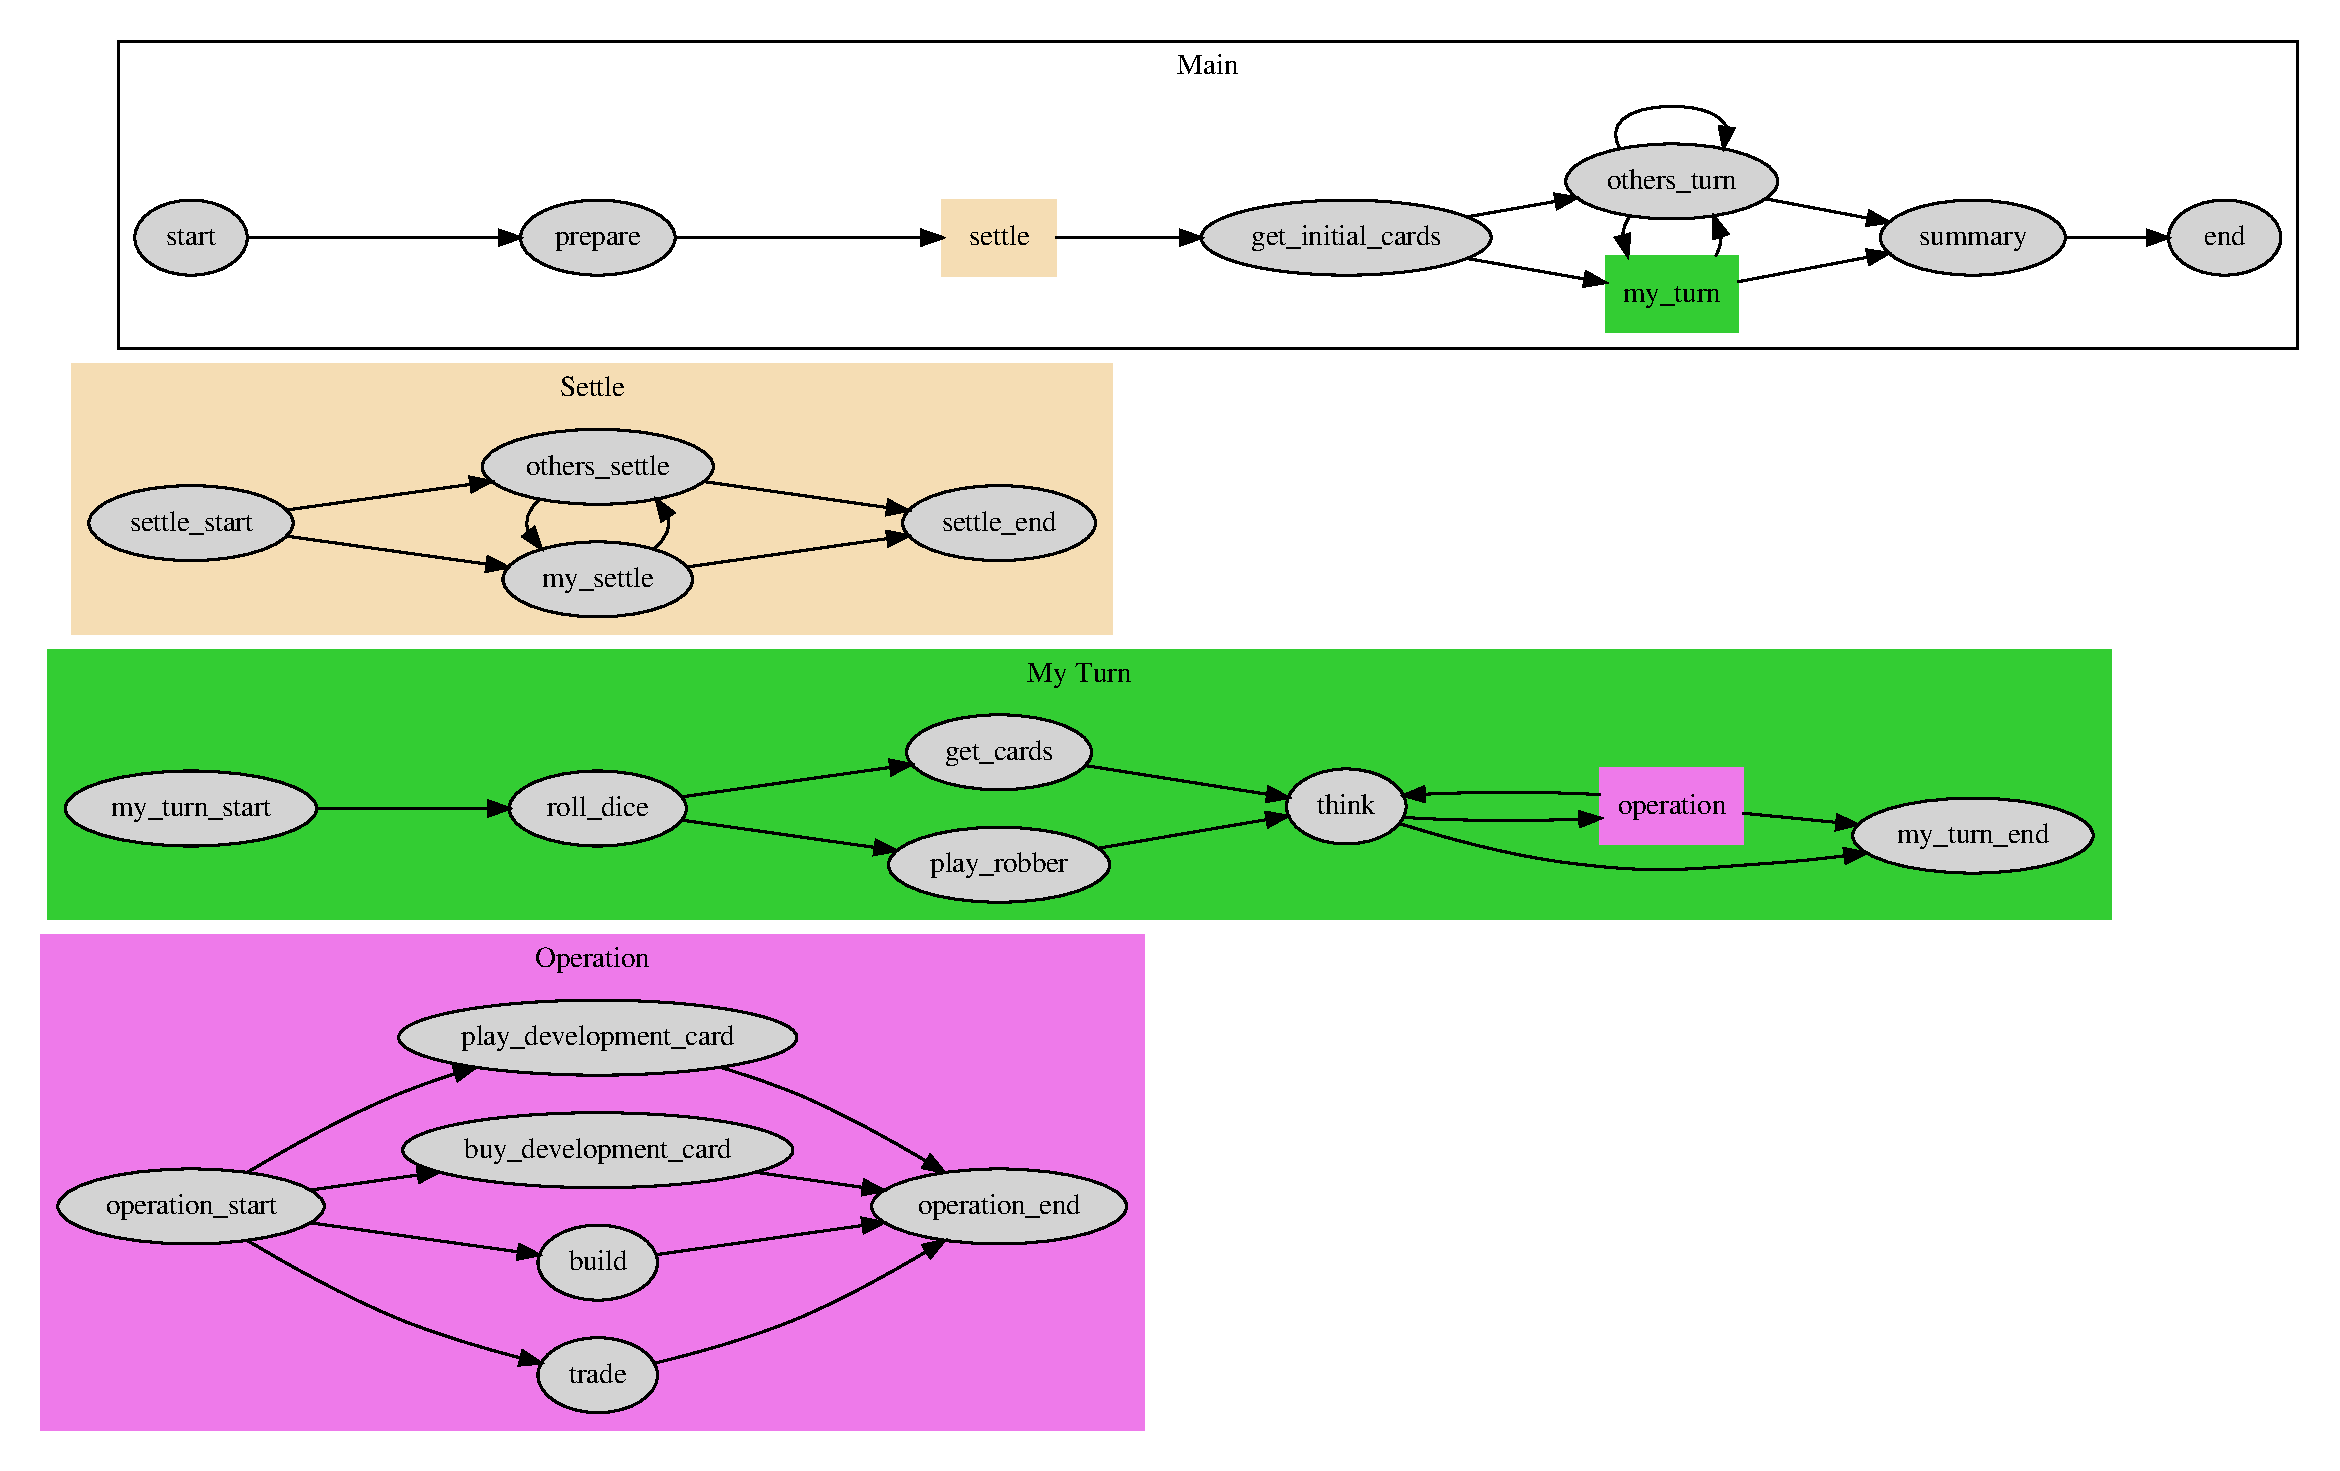
\includegraphics[max size={\textwidth}{\textheight},keepaspectratio]
{images/README/catan_web_player_state_machine.dot.eps}\caption*{卡坦岛玩家状态转换}
\end{figure} \end{center}

\section{坐标系设计}

\chapter{AI设计}

AIPlayer可以实现自动的游戏过程,一些通用的AIPlayer可以被不同的游戏重复利用。


\section{AIPlayer}
最基本的AIPlayer是随机的AIPlayer。首先根据规则,获取所有可能的Action,然后在其中随机选择一个Action返回。


\section{Evaluator}

Evaluator是对当前Board局面的一个评估函数,返回一个[0, 1]的值,0代表是最糟糕的局面,1代表是最好的局面。

通过Evaluator,我们可以获得稍好于随机操作的AIPlayer。同样的,可以首先根据规则,获取所有可能的Action。然后执行每个Action,对新的局面调用评估函数,可以得出执行哪一个Action会得到对自己最有利的局面,然后返回这个Action。

\section{MaxMinAIPlayer}

通过极大极小搜索和AlphaBeta剪枝实现多步的搜索。同样的会在搜索的尾部,调用Evaluator对局面进行评估。目前的单机搜索深度能够达到4到5层。

\section{置换表}

置换表可以用于保存某个局面的搜索评分,这样,下一次搜索到同一个局面时,可以检查是否已经有可用的评分了。通过哈希函数可以将局面映射到一个哈希键值,以及为局面加锁以防止冲突局面。

\section{历史表}

历史表对每种移动走法打分,并对打分高的的走法优先搜索,使得AlphaBeta剪枝的效率更高。本框架未实现历史表,而是通过对Action导致的新局面的评估函数作为该Action的分数进行排序。

\chapter{对弈平台}

目前尚未开始这个阶段的工作。

\chapter{TODO}

\section{基础设施}


\begin{itemize}
\item{ 平台化
\begin{itemize}
\item{ 制作游戏UI。 }
\end{itemize}
 }
\item{ Better Engineering
\begin{itemize}
\item{ 完善Readme文档。 }
\item{ Modify all assert to exception }
\end{itemize}
 }
\end{itemize}


\section{Catan}

\begin{itemize}
\item{ 前台:js/html/css + vue.js + js game engine: \href{https://github.com/craftyjs/Crafty}{Crafty}
\begin{itemize}
\item{ \href{https://github.com/collections/javascript-game-engines}{More js game engine} }
\item{ \href{https://www.youtube.com/watch?v=bI5jpueiCWw\&t=756s}{Vue.js tutorial 1} }
\item{ \href{https://www.youtube.com/watch?v=xq532yn8gMA\&t=2608s}{Vue.js turorial 2} }
\end{itemize}
 }
\item{ 后台:django
\begin{itemize}
\item{ Websocket: \href{https://www.youtube.com/watch?v=RVH05S1qab8\&list=PLcWimtlf9naWeyuY5OwQeaRNxvxTRyTCt\&index=1\&t=3148s}{tutorial} }
\end{itemize}
 }
\item{ 图片资源 }
\item{ 游戏流程 }
\end{itemize}



\section{中国象棋}


\begin{itemize}
\item{ 将中国象棋相关代码移动到一个folder下。 }
\item{ 判断和棋:长将,长捉,50步无吃子,双方无子可以过河等 }
\item{ 棋型监测:双炮,马后炮,双车错,侧面虎等。 }
\item{ 借助latex项目,实现静态棋盘的图片的生成,以及实现动态棋局gif图的生成。 }
\item{ 整理以前写的\href{https://github.com/JimmyFromSYSU/ChineseChess}{Javascript版本的象棋引擎} }
\end{itemize}


\subsection{AI设计}

AI相关内容更加复杂,需要更长时间的test,先Focus在基础设施的建设上,为AI的开发提供足够的工具集合。


\begin{itemize}
\item{ 添加Unit Test,对每个部件单独进行测试,比如player,evaluator,judge等。现在还有许多需要改进的点,每个点都建立对应的test cases。 }
\item{ 制作工具快速添加新棋局到data中。 }
\item{ 残局库:将象棋软件中的残局库添加到data中,可以通过残局对AI进行测试。 }
\item{ 加强残局能力:对将军的action优先搜索,或者对将军的局面提高评分。可以同时计算所有的控子情况。通过对局面计算所有的actions,然后对所有吃子进行加成。 }
\item{ 假设后手先走,现将后手可能的杀招计算出来,从而能够对actions的排序更加精确。 }
\item{ 如何训练和制作开局库? }
\item{ 添加多线程实现AI加速。 }
\item{ 当AI意识到自己输了的时候,AI也要选取最长路径来走。 }
\item{ MCT:
\begin{itemize}
\item{ MCT还有很多不明确的点,先确认算法,然后实现一种更加readable的版本,并对每个步骤提供足够的unit test。 }
\item{ 似乎后手的搜索不太起作用。考虑一个残局,先手优先可以吃子,但是后手可以将死先手。这时,先手陷入到了吃子的陷阱,并没有发现会被将死。测试"data/JJ象棋残局第98关.bd"。 }
\end{itemize}
 }
\item{ 实现AI的自动博弈,并计算每次结局的基本情况和整体胜率。 }
\item{ 实现训练框架对评估函数进行训练。 }
\item{ 参加中国象棋在线比赛,构建中国象棋在线比赛平台:\href{https://www.xqbase.com/protocol/cchess_ucci.htm}{UCCI 中国象棋通用引擎协议 版本:3.0} }
\end{itemize}



\section{五子棋}


\begin{itemize}
\item{ 扩展到五子棋的游戏流程。 }
\item{ 将MaxMinAIPlayer通用化,使得在五子棋等其他游戏中也可以直接复用。 }
\end{itemize}


\section{卡坦岛}

\end{document}
